\section{The Linear Complementary Filter}
\label{sec:LCF}


The complementary filter \cite{higgins1975comparison} is well known in the field of aerial robotics \cite{euston2008complementary}, for example to estimate the attitude of a quad-rotor system by combining the gyroscopic and accelerometer measurements. Unlike the Kalman filter \cite{kalman1960new} which makes no distinction between the contributions of each measurement in the frequency domain, the complementary filter exploits the influence and the accuracy of each input signal in their respective frequency domain and reconstructs the integrality of the signal by a combination of filtered measurements, with zero-phase-shift. A simple example of complementary filter is derived in Sec. \ref{subsec:cf_com_vertical}. And all along this section, we exploit the following definition:
\hspace{0.3cm}
\begin{defin}[Linear Complementary Filter] 
  We say that the transfert function $Y$ is the linear complementary filter of the transfert function $X$ if and only if $X(s) + Y(s) = 1$ for any $s \in\mathbb{C}$, $s$ being the Laplace variable. 
\end{defin}
\hspace{0.1cm}
For our case, we have three signals providing information on the CoM. (i) The first one is the geometry-based reconstruction of the CoM. It suffers mainly from biases due to modeling errors of mass distribution. It is also subject to high frequency sensor noise due to motion capture technology or the measurement of the angular position of the joints. The error between this signal and the real position of the CoM lies then in low and high frequency domains. (ii)~The second signal is the CoM acceleration extracted from force measurements. This signal suffers also from sensor noise. The double integration of this signal reduces the high frequency error but generates quadratic drift, visible in low and medium frequencies. (iii) The third signal is the ZMP, which only provides information about the horizontal position of the CoM. It contains high frequency sensor noise, but also carries error due to the linear approximation (eq. \ref{eq:lin_zmp}). This approximation assumes constant CoM height and negligible variation of the angular momentum. These assumptions are particularly acceptable in low frequency domain, specifically below natural walking rhythm. Similar reasoning concerning these measurements can be found in~\cite{schepers2009biomen,maus2011combining}. All these considerations are schematized in Figure~\ref{fig:cf-intuition}.

\begin{figure}
\begin{center}
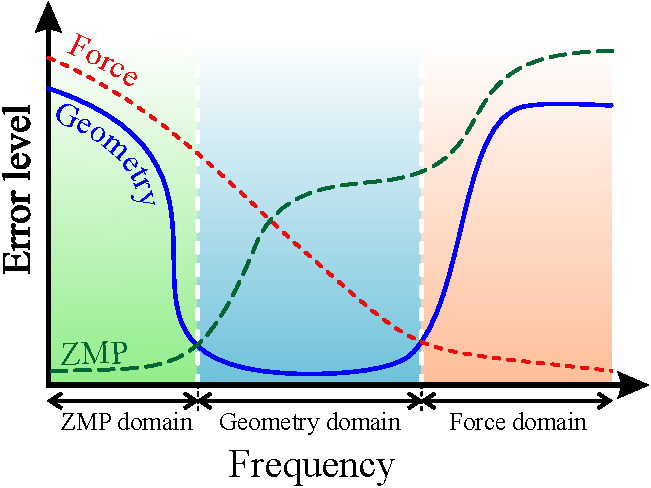
\includegraphics[width=\columnwidth]{fig/cf-intuition}
\caption{\label{fig:cf-intuition} A sketch representation of the spectral distribution of errors that would emerge from the naive reconstruction of CoM trajectory if we use only one signal (Geometry, Forces and ZMP). The signal with the lowest error is then selected at each frequency bandwidth to constitute minimal-error fusion of these signals.}
\end{center}
\end{figure}

In the following, we gradually design the complementary filters of the CoM vertical and horizontal components. We designate by $s$ the Laplace variable acting in the frequency domain. The Laplace Transform of a temporal signal $g(t)$, $t$  being the time variable, is written $G(s)$ and $sG(s)$ corresponds to the Laplace Transform of its time derivative $\dot{g}(t)$.

\subsection{Complementary filter of the CoM vertical component}
\label{subsec:cf_com_vertical}

\subsubsection{Hypothesis}
The vertical position $\bm c^{z}$ of the CoM can be observed from two decoupled sources of measurement:
\begin{itemize}
  \item (1) the mass distribution of the anthropomorphic system coupled with the current measure of the links' position provide an estimation $\tilde{\bm c}^z$
  \item (2)  vertical contact force measurements divided by the mass  $m$ and subtracted from gravity (cf. Newton equation (\ref{eq:linear_momentum})) provide estimation $\tilde{\ddot{\bm c}}^{z}$ of the vertical acceleration of the CoM. 
\end{itemize}
The complementary filter diagram corresponding to those two measurements is shown in Figure \ref{fig:cf_com_vertical}. $H_{1}^z$ and $H_{2}^z$ are the linear filters of $\tilde{\bm c}^{z}$ and $\tilde{\ddot{\bm c}}^{z}$ respectively.

\begin{figure}
\begin{center}
%\tikzstyle{block} = [draw, fill=blue!20, rectangle, 
%    minimum height=2em, minimum width=3em]
%\tikzstyle{sum} = [draw, fill=blue!20, circle, node distance=1cm]
%\tikzstyle{input} = [coordinate]
%\tikzstyle{output} = [coordinate]
%\tikzstyle{pinstyle} = [pin edge={to-,thin,black}]
%
%% The block diagram code is probably more verbose than necessary
%\begin{tikzpicture}[auto, node distance=1.2cm,>=latex']
%    % We start by placing the blocks
%    \node [input, name=input1] {};
%    \node [input, name=input2, below of = input1] {};
%    \node [block, right of=input1, node distance = 1.2cm] (H1) {$H_{1}$};
%    \node [block, below of = H1] (H2) {$H_{2}$};
%    \node [sum, right= 1.2cm of {$(H1)!0.5!(H2)$}] (sum) {};
%   
%    % Once the nodes are placed, connecting them is easy. 
%    \draw [draw,->] (input1) -- node[pos=0.2] {$\bm c^{z}$} (H1);
%    \draw [draw,->] (input2) -- node[pos=0.2] {$\bm \ddot{c}^{z}$} (H2);
%    \draw [draw,->] (H1.east) -| node[pos=0.99] {$$}  node [near end] {} (sum);
%    \draw [draw,->] (H2.east) -| node[pos=0.99] {$$}  node [near end] {} (sum);
%    \draw [draw,->] (sum) -- node {$\bm c^{z}_{\text{est}}$} +(1,0);
%\end{tikzpicture}
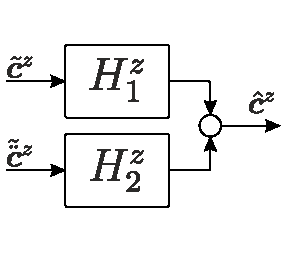
\includegraphics[width=0.35\columnwidth]{fig/block-diagram-z}\hspace{0.1\columnwidth}
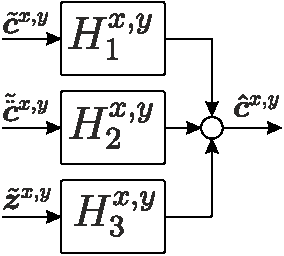
\includegraphics[width=0.35\columnwidth]{fig/block-diagram-x-y}

\end{center}
\caption{On the left, diagram of the complementary filter for the CoM vertical component. On the right, the diagram for the horizontal components.}
\label{fig:cf_com_vertical}
\end{figure}

\subsubsection{Design}
For the first signal, the noise is mostly located in the high frequency domain. While for the second measurement, due to the double integration process, the noise is mainly concentrated in the low frequency domain. Then $s^{2}H_{2}^z$~\footnote{the $s^{2}$ term before $H_{2}^z$ comes directly from the fact that $s^{2}\bm C^{z}(s)$ is the Laplace Transform of $\bm \ddot{c}^{z}$.}
is made a high-pass filter in order to filter out the low frequency noise in the double integration processus. We can now set:
\begin{equation}
  s^{2}H^{z}_{2} (s) = \frac{{(s\tau_{1})}^{2}}{(1+s\tau_{1})^{2}},
  \label{eq:z_filter1}
\end{equation}
with $\tau_{1} \overset{\text{def}}{=} \frac{1}{2 \pi f_{1}}$~\footnote{in the previous section \ref{sec:dynamics}, the bold $\bm \tau$ means the moment of the contact forces wrench. In the current section, $\tau$ refers to the inverse pulsation in the context of linear filtering.} the inverse pulsation and $f_{1}$ the cut-off frequency of the high-pass filter $H_{2}$. Therefore
(\ref{eq:z_filter1}) is equivalent to:
\begin{equation}
  H_{2}^{z} (s) = \frac{{\tau_{1}}^{2}}{(1+s\tau_{1})^{2}}
\end{equation}
Accordingly, $H_{1}$ can be directly computed as the complement of $s^{2}H_{2}$, i.e. $H_{1} \overset{\text{def}}{=}  1 - s^{2}H_{2}$. So $H_{1}$ is of the following form:
\begin{equation}
  H_{1}^{z} (s) = \frac{1 + 2s\tau_{1}}{(1+s\tau_{1})^{2}},
\end{equation}
which is the combination of a low-pass filter and a bandpass filter, both with a unique cutting frequency of value $f_{1}$. As expected, $H_{1}$ acts in the low frequency domain. Figure \ref{fig:bd_z} represents the bode diagram of the two designed filters $H_{1}$ and $H_{2}$.

 \begin{figure}
       \begin{center}
               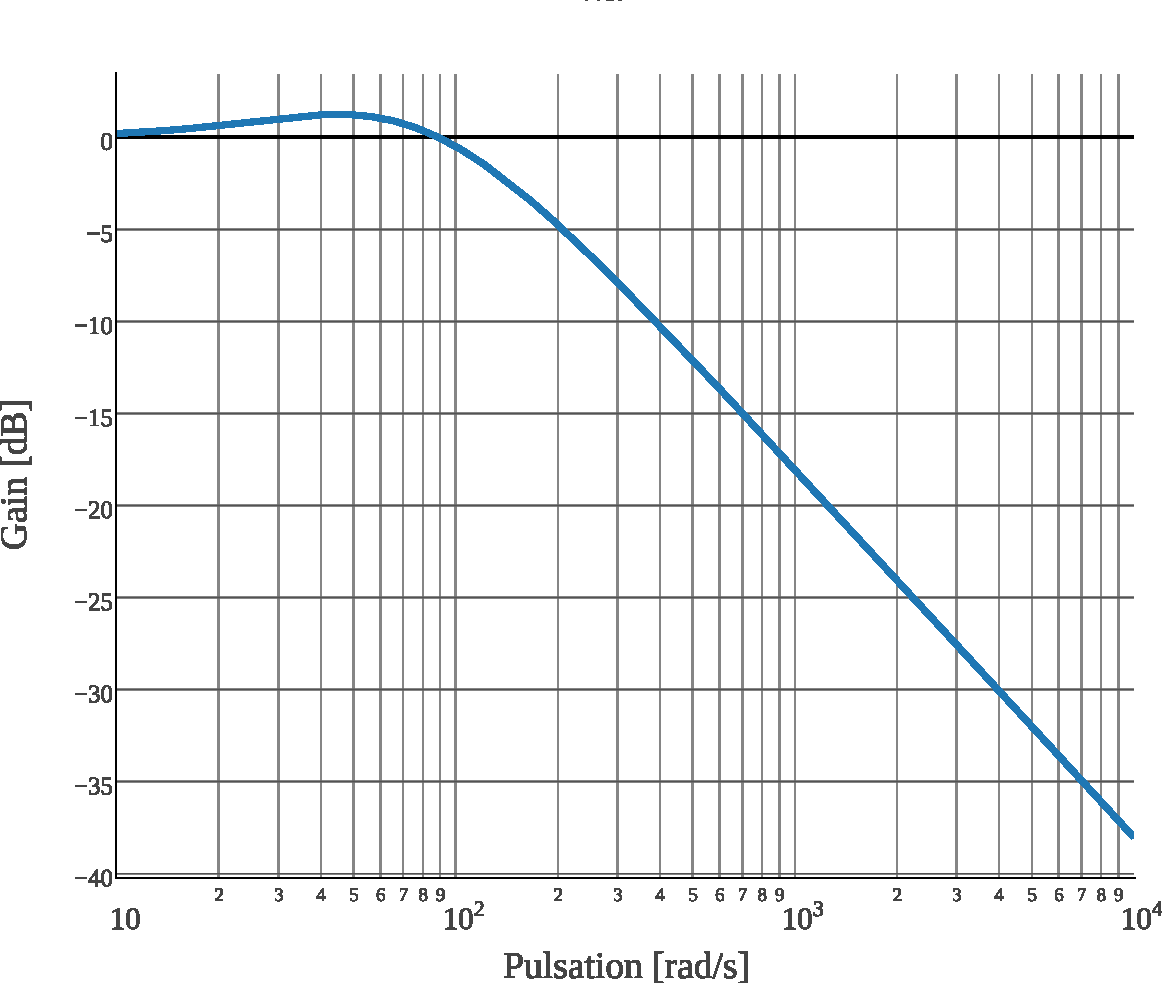
\includegraphics[width=0.49\columnwidth]{fig/H1_z}
               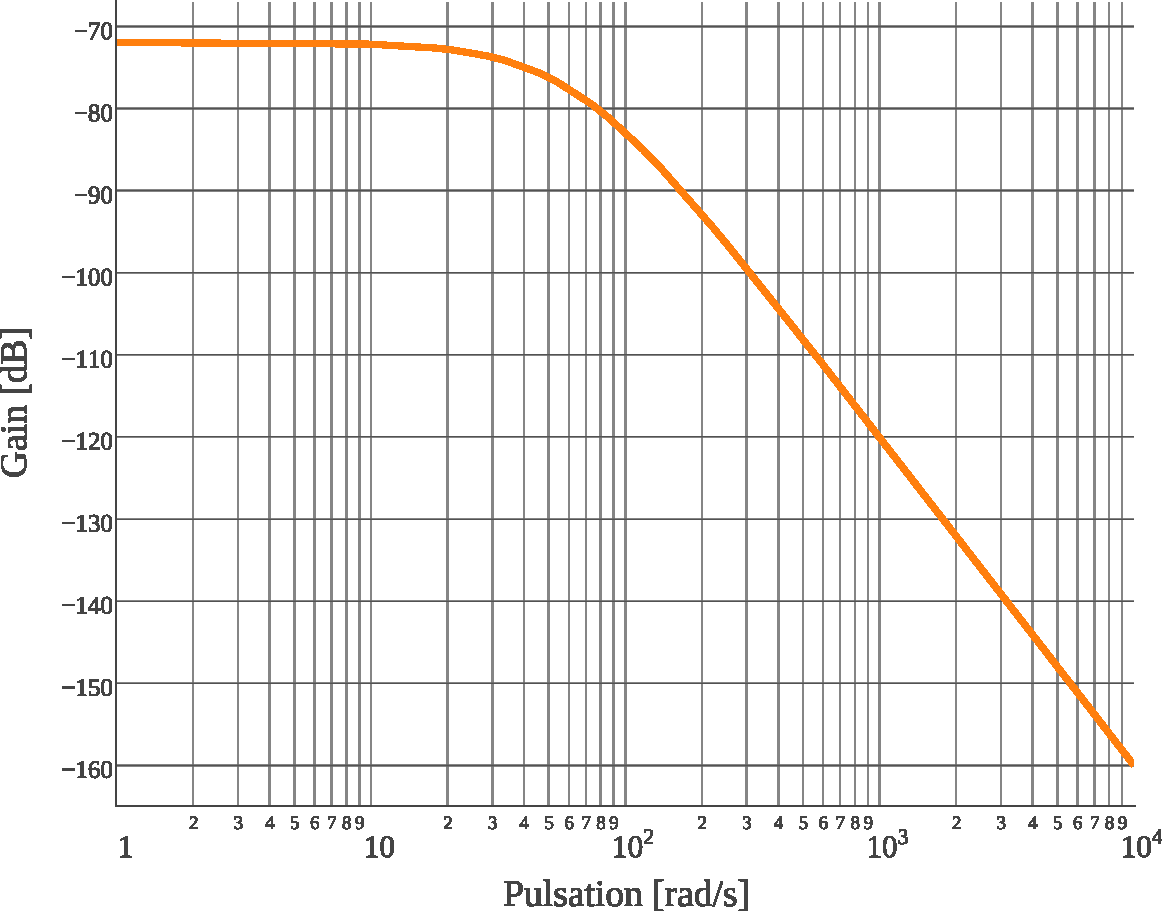
\includegraphics[width=0.49\columnwidth]{fig/H2_z}
       \end{center}
       \caption{Bode diagram of filter $H^{z}_{1}$ (left) and $H^{z}_{2}$ (right) with \mbox{$f_{1} = 10$ Hz.}}
       \label{fig:bd_z}
 \end{figure}

One can remark that both filters depends on the same free variable $f_{1}$, which corresponds to the unique cutting frequency of the low-pass and high-pass filters. The choice of $f_{1}$ corresponds to the frequency of sensor noise in the force measurement and link position reconstruction.

\subsubsection*{Remark} Due to the presence of double integrator in the acceleration measurements, the order of the filter has to be at least 2. Otherwise, the filter $H_2^z$ would be unstable.
 
\subsection{Complementary filter of the CoM horizontal components}

In the case of horizontal components estimation, we add (iii) the measure of the  ZMP position to the input of the estimator. The complete diagram of the complementary filter of horizontal components is depicted in Figure \ref{fig:cf_com_vertical}.

\subsubsection{Hypothesis}
The hypotheses of the CoM vertical component still hold for the case of the horizontal ones. Concerning the ZMP, we make the hypothesis that the ZMP is a good approximation of the CoM position at a very low frequency level. 

\subsubsection{Design}

We first write the Laplace Transform of (\ref{eq:lin_zmp}):
\begin{equation}
  \bm{Z}^{x,y} (s) = \left(1 -  \tau_{z}^{2} s^{2}\right) \bm C^{x,y} (s),
  \label{eq:lt_zmp}
\end{equation}
with $\tau_{z} \overset{\text{def}}{=} \sqrt{\frac{\bm c^{z}}{\bm g^{z}}}$ the inverse pulsation of the linearized ZMP model. (\ref{eq:lt_zmp}) can be rewritten as:
\begin{equation}
  \bm{Z}^{x,y} (s) = \left(1 +  \tau_{z}s\right) \left(1 -  \tau_{z}s\right) \bm C^{x,y} (s)
  \label{eq:lt_zmp2}
\end{equation}

By looking at (\ref{eq:lt_zmp2}), one can remark that the ZMP dynamics is composed of a stable and unstable component. In the following, we then have to reject the unstable dynamic in order to make the complementary filter stable. So, we want that:
\begin{equation}
  H^{x,y}_{3} (s) (1 + \tau_{z}s)(1 - \tau_{z}s)= \frac{1 - \tau_{z}s}{(1+s\tau_{2})^{2}},
  \label{eq:zmp_filter1}
\end{equation}
with $\tau_{2} \overset{\text{def}}{=} \frac{1}{2 \pi f_{2}}$ the inverse pulsation and $f_{2}$ the cutting frequency of the low-pass filter of the horizontal ZMP components. $H^{x,y}_{3}$ has the following expression:
\begin{equation}
  H^{x,y}_{3} (s) = \frac{1}{(1+s\tau_{2})^{2}(1 + \tau_{z}s)}
  \label{eq:zmp_filter2}
\end{equation}

While $H^{x,y}_{2}$ remains unchanged and equal to $H^{z}_{2}$, $H^{x,y}_{1}$ is the complementary filter of both $s^{2}H^{x,y}_{2}$ and \mbox{$(1 + \tau_{z}s)(1 - \tau_{z}s)H^{x,y}_{3}$} transfert function, leading to:
\begin{align} 
  H^{x,y}_{1}(s) &= 1 - s^{2}H^{x,y}_{2}(s) - (1 + \tau_{z}s)(1 - \tau_{z}s)H^{x,y}_{3}(s)\nonumber
  \\&= 1 - \frac{{(s\tau_{1})}^{2}}{(1+s\tau_{1})^{2}} - \frac{1 - \tau_{z}s}{(1+s\tau_{2})^{2}}
\end{align}

Figure \ref{fig:bd_xy} illustrates the bode diagrams of the designed filter  $H^{x,y}_{1}$ and $H^{x,y}_{3}$. We can remark that $H^{x,y}_{1}$ acts as a bandpass filter in a bandwidth around $\left[f_{2}; f_{1} \right]$, while $H^{x,y}_{3}$ is mainly a third order low-pass filter because the chosen value of $\tau_{2}$ is very closed to $\tau_{z}$.
\begin{figure}
  \begin{center}
    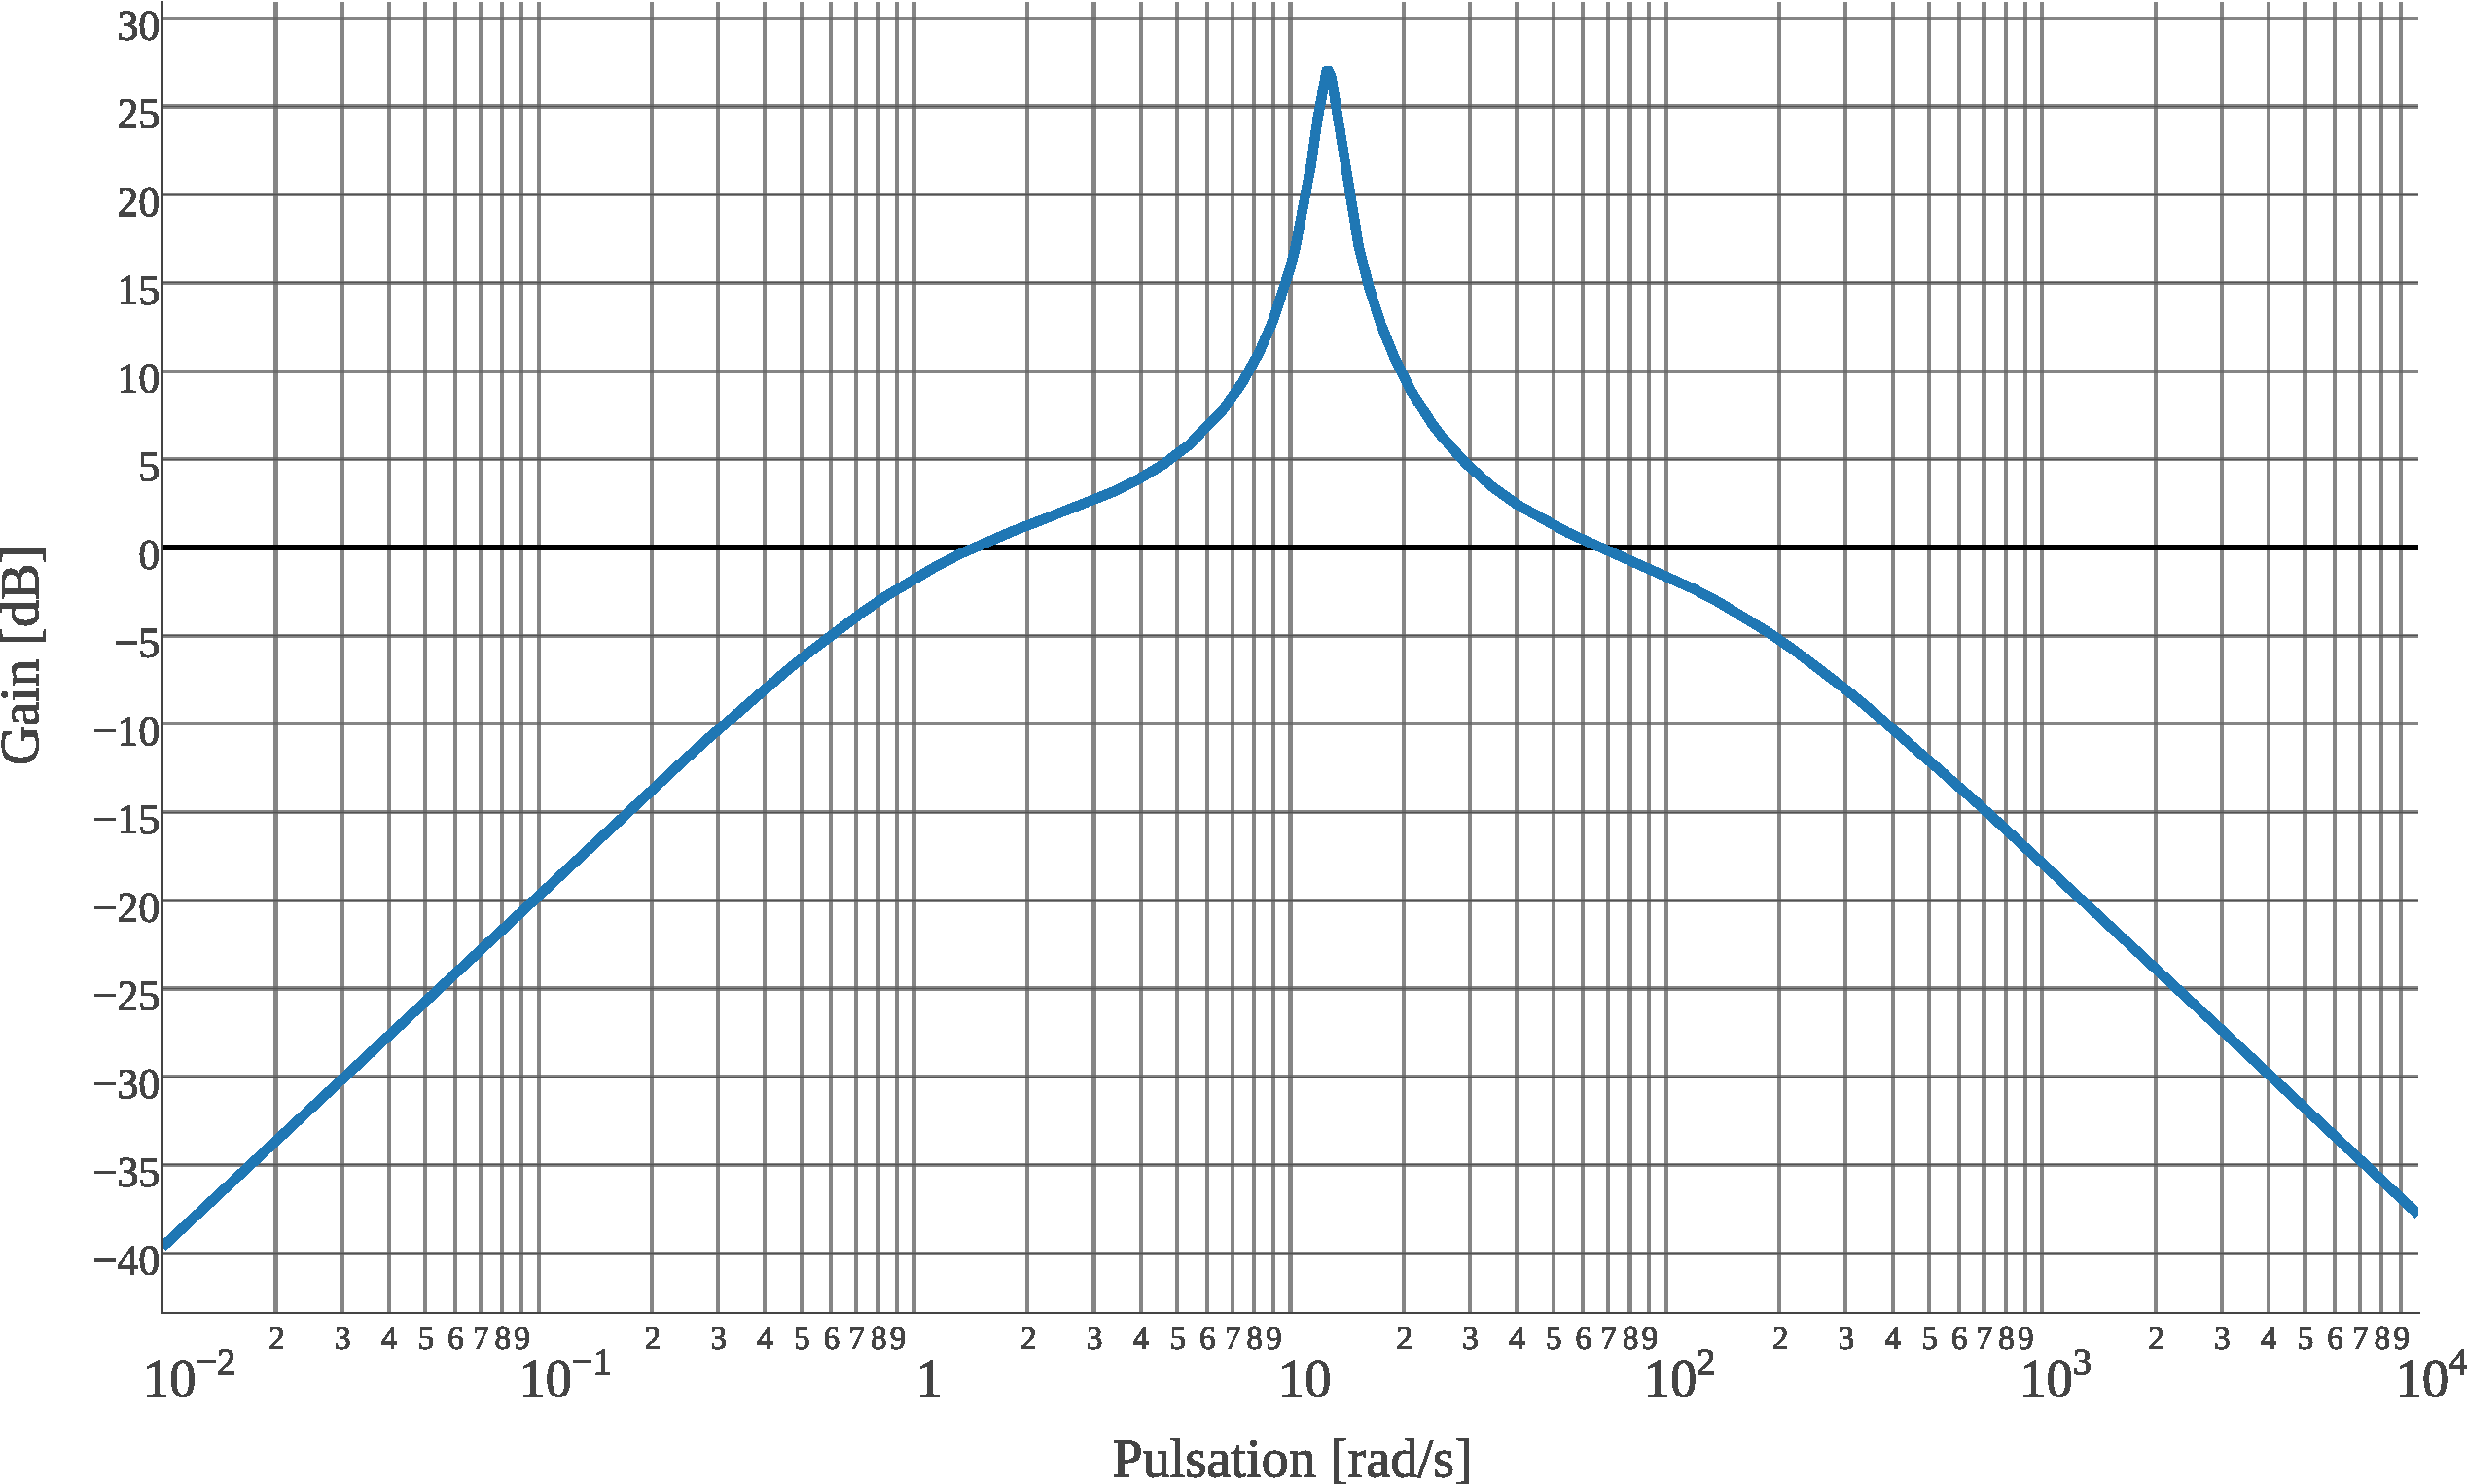
\includegraphics[width=0.54\columnwidth]{fig/H1_xy}
    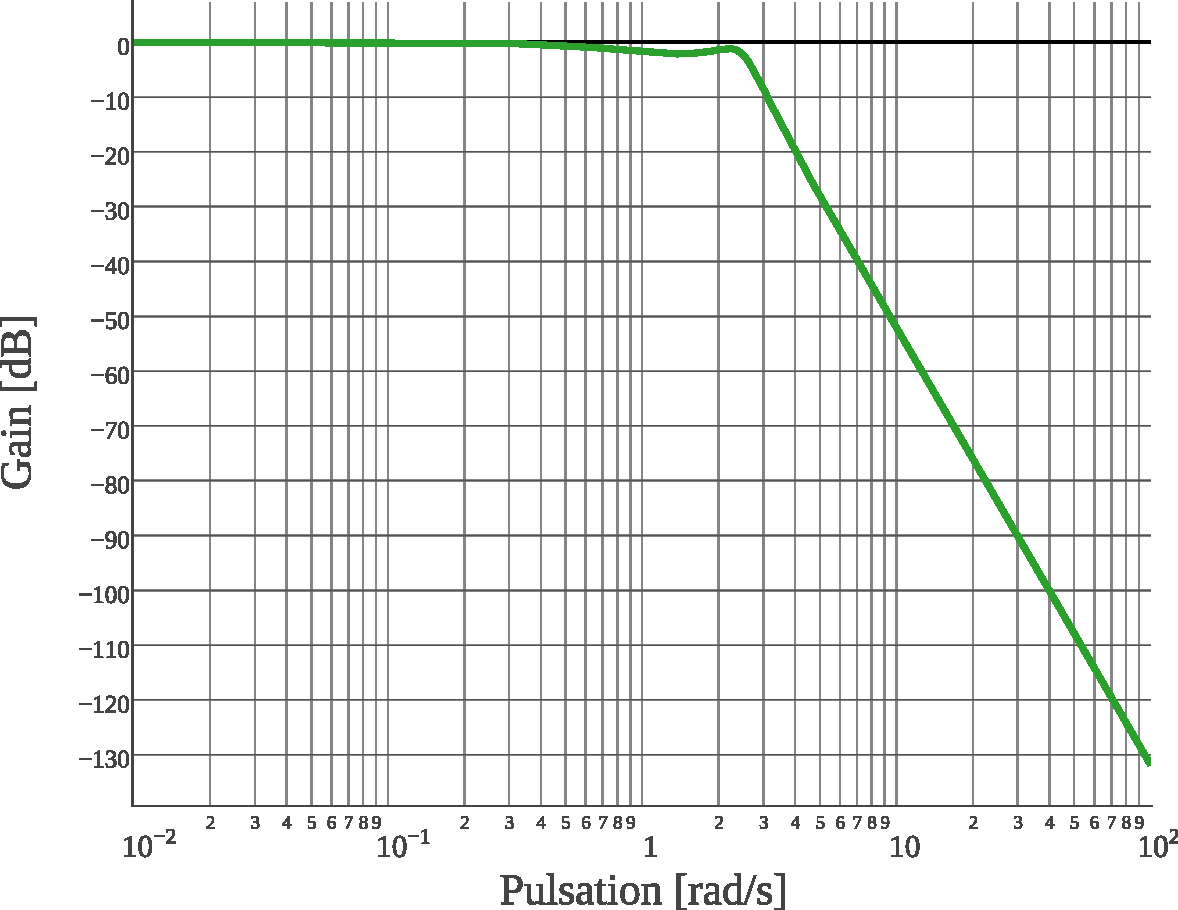
\includegraphics[width=0.44\columnwidth]{fig/H3_xy}
  \end{center}
  \caption{Bode diagram of filter $H^{x,y}_{1}$ (left) and $H^{x,y}_{3}$ (right) with \mbox{$f_{1} = 10$ Hz}, $f_{2} = 0.4$ Hz and $\bm c^{z} = 0.6$ m. $H^{x,y}_{2}$ Bode diagram is the same as in Figure~\ref{fig:bd_z}}
  \label{fig:bd_xy}
\end{figure}

Choosing the frequency $f_{2}$ is a little bit more subtile than in the case of $f_{1}$. We consider that the linearized ZMP model is only valid for the frequencies below the fondamental frequency of the locomotion pattern. In general, this fondamental frequency is around $1$ or $2$ Hz. Therefore, we might consider a value of $f_{2}$ below $1$ Hz. 
